\section{Machine Learning Library}
\subsubsection{hive.sql}
\begin{frame}[fragile]
\frametitle{Machine Learning Library}
\begin{itemize}
\item Spark Machine Learning Library - {\color{mycolordef}MLlib} - is a distributed machine learning framework on top of Spark
\item MLlib has RDD and DataFrame APIs
\item RDD API is now in maintenance mode: bugs are fixed, no new features are added
\item DataFrame API is catching up, once it does, RDD API will be removed
\item Many common machine learning and statistical algorithms have been implemented and are shipped with MLlib which simplify large scale machine learning pipelines, including:
  \begin{itemize}
    \item summary statistics, correlations, sampling, hypothesis testing
    \item classification and regression: support vector machines, logistic regression, linear regression, decision trees, naive Bayes classification
    \item cluster analysis methods including k-means
    \item dimensionality reduction techniques such as SVD and PCA
    \item feature extraction and transformation functions
    \item optimization algorithms such as stochastic gradient descent
  \end{itemize}
\end{itemize}
\end{frame}

\subsection{Lab 5}
\subsubsection{Logistic Regression}
\begin{frame}[fragile]
\frametitle{Lab 5: Logistic Regression}
\begin{itemize}
\item In this lab we have a training set consisting of class label (0 or 1) and 692 numerical features
\item The data is sparse and is given in libsvm format in {\color{mycolorcli}\verb|data/sample_libsvm_data.txt|}
\item Linear regression model tries to predict the class $y$ based on features 
  $x_i$ as follows:
  \begin{equation*}
    y = \frac{1}{1 + e^{-(\sum_{i}{w_i x_i} + b)}} 
  \end{equation*}
  where $w_i$ and $b$ are parameters that the model needs to learn to minimize error on the given training set. 
  \item After the model is trained, the parameters are printed. 
  \item Since most of them are zero, sparse format is used.
\end{itemize}
\end{frame}


\begin{frame}[fragile]
\frametitle{Lab 5: Logistic Regression}
{\small
{\color{mycolorcode}
\begin{verbatim}
from pyspark.sql import SparkSession
from pyspark.ml.classification import LogisticRegression

spark = SparkSession.builder.getOrCreate()

# Load training data
training = spark.read.format("libsvm").\
                 load("data/sample_libsvm_data.txt")
lr = LogisticRegression(maxIter=10, 
                   regParam=0.3, elasticNetParam=0.8)
# Fit the model
lrModel = lr.fit(training)

# Print the coefficients and intercept for logistic regression
print("Coefficients: " + str(lrModel.coefficients))
print("Intercept: " + str(lrModel.intercept))
\end{verbatim}
}
}
\end{frame}

\subsubsection{Perceptron}
\begin{frame}[fragile]
\frametitle{Lab 5: Perceptron}
\begin{columns}
\begin{column}{.75\textwidth}
\begin{itemize}
\item The data has 3 classes and 4 features and is given in libsvm format 
  {\small{\color{mycolorcli}\verb|data/sample_multiclass_classification_data.txt|}}
\item The model is a fully connected neural network with 4 layers.
\item \verb|60%| of data is used as training set and \verb|40%| as validation set.
\item 100 epochs is used for training, mini-batch size is 128.
\item Prediction accuracy on the validation set is printed: \verb|90%|.
\end{itemize}
\end{column}

\begin{column}{.25\textwidth}
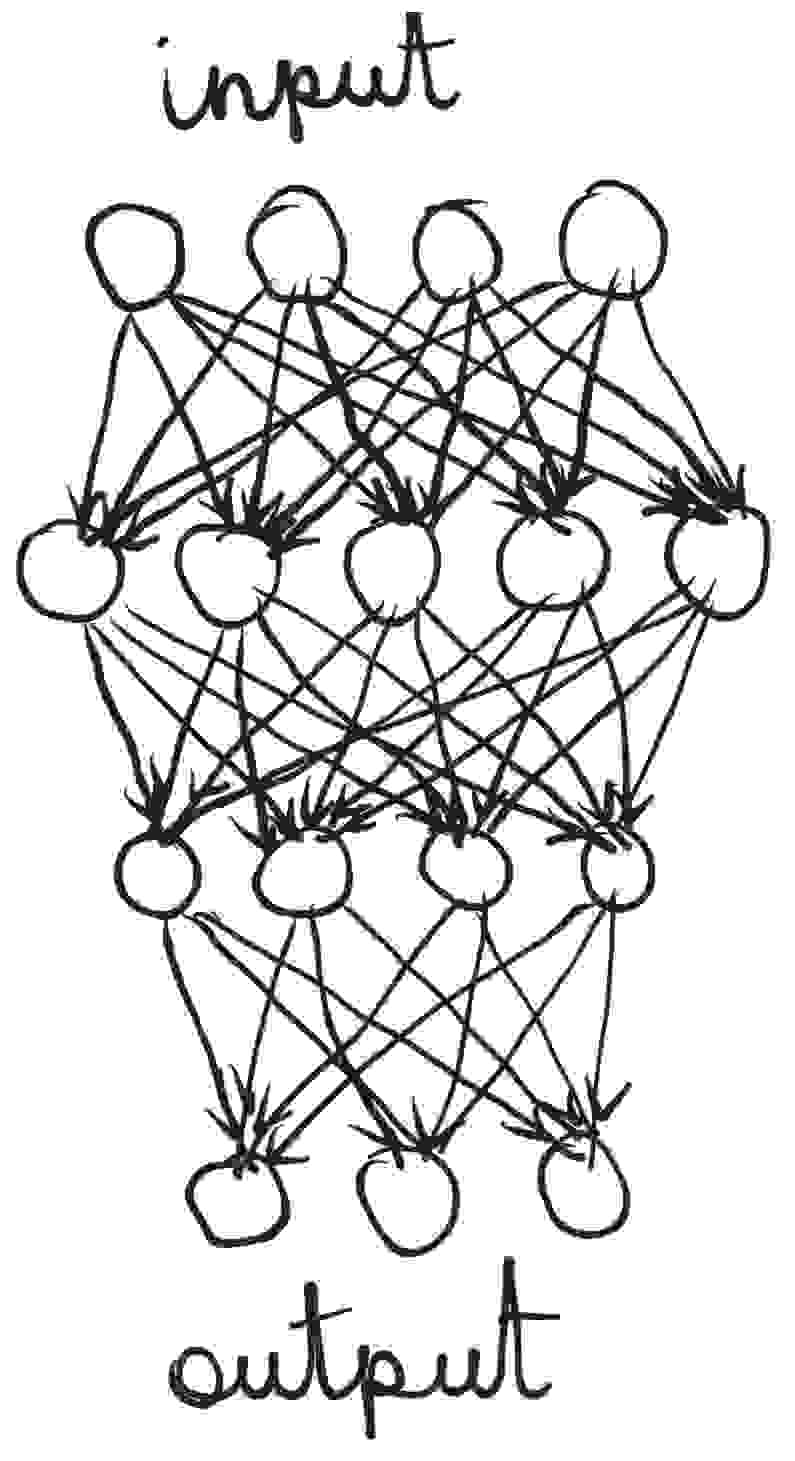
\includegraphics[width=3cm]{graphs/perceptron.jpg}
\end{column}


\end{columns}

\end{frame}


\begin{frame}[fragile]
\frametitle{Lab 5: Perceptron}
{\small
{\color{mycolorcode}
\begin{verbatim}
from pyspark.ml.classification 
     import MultilayerPerceptronClassifier as mlp
from pyspark.ml.evaluation 
     import MulticlassClassificationEvaluator as mce
spark = SparkSession.builder.getOrCreate()
data = spark.read.format("libsvm")\
    .load("data/sample_multiclass_classification_data.txt")
splits = data.randomSplit([0.6, 0.4], 1234)
train = splits[0]; test = splits[1]
layers = [4, 5, 4, 3]
trainer = mlp(maxIter=100, layers=layers, blockSize=128, seed=1234)
model = trainer.fit(train)
result = model.transform(test)
predictionAndLabels = result.select("prediction", "label")
evaluator = mce(metricName="accuracy")
print(evaluator.evaluate(predictionAndLabels))))
\end{verbatim}
}
}
\end{frame}
